\label{2.5 C5M Answer Key}
\subsection{Answer Key}
\tiny
\renewcommand{\insertclass}{- Class 5}
\renewcommand{\insertsubject}{ - Math}

\begin{frame}[shrink=0.1,label=QPC5QC5BM - BM - Q16]{Q1 [Basic Math]}
\vspace{-0.2cm}
\mcqimgleftFourOne{
questionnumber={1}, 
questionTag={C5BM - BM - Q16}, 
questiontext={Subtract.},
imgtabletikz  = {
\begin{table}[H]
\centering
\begin{tabular}{cccc}
& 9 & 8 &6  \\
$-$ & 6 & 9 & 9\\
\hline
& & & \\
\hline
\end{tabular}
\end{table} },
optionA={313},
optionB={1685},
optionC={ 287},
optionD={397},
correctoption={C},
leftmini={0.5},
rightmini={0.4},
}


\begin{minipage}{\linewidth}
\hspace{1cm}
\centering
\tiny
\renewcommand{\arraystretch}{1.25}
\begin{tabular}{|M{1.2cm}|M{0.8cm}|M{0.8cm}|M{0.8cm}|M{0.8cm}|M{0.8cm}|}
\hline
Option & A (\ding{55}) & B (\ding{55}) & \cellcolor{cellgreen} C (\ding{51}) & D (\ding{55}) & E \\ 
\hline
5 A & \highno{24\%} & \highno{0\%} & \highgreen{76\%} & \highno{0\%} & \highno{0\%} \\ 
 \hline 
5 B & \highno{7\%} & \highno{7\%} & \highgreen{79\%} & \highno{7\%} & \highno{0\%} \\ \hline
\end{tabular}
\end{minipage}

\end{frame}
% \input{4. PPT/My Answer/Math/C5/117_C5M - Q1}


\begin{frame}[shrink=0.1,label=QPC5QC5BM - BM - Q21]{Q2 [Basic Math]}
\vspace{-0.2cm}
\mcqtextbottomOneFour{
questionnumber={2}, 
questionTag={C5BM - BM - Q21}, 
questiontext={How many digits are greater than 3? \quad 		12667322},
optionA={4},
optionB={8},
optionC={3},
optionD={0},
correctoption={C},}

\begin{minipage}{\linewidth}
\hspace{1cm}
\centering
\tiny
\renewcommand{\arraystretch}{1.25}
\begin{tabular}{|M{1.2cm}|M{0.8cm}|M{0.8cm}|M{0.8cm}|M{0.8cm}|M{0.8cm}|}
\hline
Option & A (\ding{55}) & B (\ding{55}) & \cellcolor{cellgreen} C (\ding{51}) & D (\ding{55}) & E \\ 
\hline
5 A & \highno{6\%} & \highno{18\%} & \highno{65\%} & \highno{6\%} & \highno{6\%} \\ 
 \hline 
5 B & \highno{7\%} & \highno{7\%} & \highgreen{79\%} & \highno{0\%} & \highno{7\%} \\ \hline
\end{tabular}
\end{minipage}

\end{frame}
% \input{4. PPT/My Answer/Math/C5/117_C5M - Q2}


\begin{frame}[shrink=0.1,label=QPC5QC6M01 - DT - Q7]{Q5 [Basic Math]}
\vspace{-0.2cm}
\mcqtextbottomOneFour{
questionnumber={5}, 
questiontext={Find the remainder of the following. \quad 19477 $\divisionsymbol$ 9 },
optionA={1},
optionB={0},
optionC={2164},
optionD={2184},
questionTag={C6M01 - DT - Q7}, 
correctoption={A},
}

\begin{minipage}{\linewidth}
\hspace{1cm}
\centering
\tiny
\renewcommand{\arraystretch}{1.25}
\begin{tabular}{|M{1.2cm}|M{0.8cm}|M{0.8cm}|M{0.8cm}|M{0.8cm}|M{0.8cm}|}
\hline
Option & \cellcolor{cellgreen} A (\ding{51}) & B (\ding{55}) & C (\ding{55}) & D (\ding{55}) & E \\ 
\hline
5 A & \highred{24\%} & \highno{12\%} & \highno{29\%} & \highno{18\%} & \highno{18\%} \\ 
 \hline 
5 B & \highno{57\%} & \highno{7\%} & \highno{21\%} & \highno{7\%} & \highno{7\%} \\ \hline
\end{tabular}
\end{minipage}

\end{frame}
% \input{4. PPT/My Answer/Math/C5/117_C5M - Q5}


\begin{frame}[shrink=0.1,label=QPC5QC6M01 - DT - Q6]{Q10 [Basic Math]}
\vspace{-0.2cm}
\mcqimgleftFourOne{
questionnumber={10}, 
questiontext={Add. },
imgtabletikz  = {  
\renewcommand{\arraystretch}{1.5}
\begin{tabular}{cccccc}
  & 8 & 2 & 5 & 7 & 0  \\
 + & 5 & 8 & 3 & 2 & 0 \\
 \hline
 &&&&&\\
 \hline
\end{tabular} },
optionA={1310890},
optionB={140980},
optionC={140890},
optionD={14890},
questionTag={C6M01 - DT - Q6},
leftmini={0.5},
rightmini={0.4},
correctoption={C},
}

\begin{minipage}{\linewidth}
\hspace{1cm}
\centering
\tiny
\renewcommand{\arraystretch}{1.25}
\begin{tabular}{|M{1.2cm}|M{0.8cm}|M{0.8cm}|M{0.8cm}|M{0.8cm}|M{0.8cm}|}
\hline
Option & A (\ding{55}) & B (\ding{55}) & \cellcolor{cellgreen} C (\ding{51}) & D (\ding{55}) & E \\ 
\hline
5 A & \highno{0\%} & \highno{0\%} & \highgreen{94\%} & \highno{6\%} & \highno{0\%} \\ 
 \hline 
5 B & \highno{7\%} & \highno{7\%} & \highgreen{86\%} & \highno{0\%} & \highno{0\%} \\ \hline
\end{tabular}
\end{minipage}

\end{frame}
% \input{4. PPT/My Answer/Math/C5/117_C5M - Q10}


\begin{frame}[shrink=0.1,label=QPC5QC6M04 - DT - Q1]{Q35 [Basic Math]}
\vspace{-0.2cm}
\mcqimgleftFourOne{
questionnumber={35}, 
questiontext={Find the image with an odd number count.},
imgtabletikz  = {

\tikzset{every picture/.style={line width=0.75pt,scale=\scalefactor}} 
\begin{tikzpicture}[x=0.75pt,y=0.75pt,yscale=-1,xscale=1]
\draw (178.5,110.5) node  {\adjustbox{scale=\scalefactor}{\includegraphics[width=80pt,height=60pt]{C6M04 - DT - Q1i.png}}};
\draw (374.5,109.5) node  {\adjustbox{scale=\scalefactor}{\includegraphics[width=80pt,height=60pt]{C6M04 - DT - Q1ii.png}}};
\draw (90,155) node [anchor=north west][inner sep=0.75pt]   [align=left] {Number of balls = \rule{40pt}{0.5pt}};
\draw (295,155) node [anchor=north west][inner sep=0.75pt]   [align=left] {Number of dogs = \rule{40pt}{0.5pt}};
\end{tikzpicture}  
},
optionA={Balls},
optionB={Dogs},
optionC={Both balls and dogs},
optionD={None of these},
questionTag={C6M04 - DT - Q1}, 
leftmini={0.5},
rightmini={0.35},
correctoption={B},
}

\begin{minipage}{\linewidth}
\hspace{1cm}
\centering
\tiny
\renewcommand{\arraystretch}{1.25}
\begin{tabular}{|M{1.2cm}|M{0.8cm}|M{0.8cm}|M{0.8cm}|M{0.8cm}|M{0.8cm}|}
\hline
Option & A (\ding{55}) & \cellcolor{cellgreen} B (\ding{51}) & C (\ding{55}) & D (\ding{55}) & E \\ 
\hline
5 A & \highno{12\%} & \highno{65\%} & \highno{6\%} & \highno{6\%} & \highno{12\%} \\ 
 \hline 
5 B & \highno{29\%} & \highno{50\%} & \highno{14\%} & \highno{0\%} & \highno{7\%} \\ \hline
\end{tabular}
\end{minipage}

\end{frame}
% \input{4. PPT/My Answer/Math/C5/117_C5M - Q35}


\begin{frame}[shrink=0.1,label=QPC5QC5M01 - DT - Q6]{Q4 [1. Number System*]}
\vspace{-0.2cm}
\mcqtextbottomOneFour{
questionnumber={4}, 
questionTag={C5M01 – DT – Q6},  
questiontext={Express the following in numbers.\\
\hspace{2cm}Four thousand nine hundred and two. },
optionA={492},
optionB={49002},
optionC={4092},
optionD={4902},
correctoption={D},
}

\begin{minipage}{\linewidth}
\hspace{1cm}
\centering
\tiny
\renewcommand{\arraystretch}{1.25}
\begin{tabular}{|M{1.2cm}|M{0.8cm}|M{0.8cm}|M{0.8cm}|M{0.8cm}|M{0.8cm}|}
\hline
Option & A (\ding{55}) & B (\ding{55}) & C (\ding{55}) & \cellcolor{cellgreen} D (\ding{51}) & E \\ 
\hline
5 A & \highno{18\%} & \highno{6\%} & \highno{6\%} & \highno{71\%} & \highno{0\%} \\ 
 \hline 
5 B & \highno{0\%} & \highno{29\%} & \highno{21\%} & \highno{50\%} & \highno{0\%} \\ \hline
\end{tabular}
\end{minipage}

\end{frame}
% \input{4. PPT/My Answer/Math/C5/117_C5M - Q4}


\begin{frame}[shrink=0.1,label=QPC5QC5M01 - DT - Q7]{Q12 [1. Number System*]}
\vspace{-0.2cm}
\mcqtextbottomOneFour{
questionnumber={12}, 
questionTag={C5M01 – DT – Q7},  
questiontext={Arrange the following numbers in descending order.\\ \medskip
\hspace{4cm}367, 376, 389, 498 },
optionA={367, 376, 389, 498},
optionB={498, 389, 376, 367},
optionC={389, 498, 367, 376},
optionD={376, 399, 389, 367},
correctoption={B},
}

\begin{minipage}{\linewidth}
\hspace{1cm}
\centering
\tiny
\renewcommand{\arraystretch}{1.25}
\begin{tabular}{|M{1.2cm}|M{0.8cm}|M{0.8cm}|M{0.8cm}|M{0.8cm}|M{0.8cm}|}
\hline
Option & A (\ding{55}) & \cellcolor{cellgreen} B (\ding{51}) & C (\ding{55}) & D (\ding{55}) & E \\ 
\hline
5 A & \highno{6\%} & \highgreen{88\%} & \highno{6\%} & \highno{0\%} & \highno{0\%} \\ 
 \hline 
5 B & \highno{29\%} & \highno{50\%} & \highno{14\%} & \highno{0\%} & \highno{7\%} \\ \hline
\end{tabular}
\end{minipage}

\end{frame}
% \input{4. PPT/My Answer/Math/C5/117_C5M - Q12}


\begin{frame}[shrink=0.1,label=QPC5QC5M01 - DT - Q10]{Q15 [1. Number System*]}
\vspace{-0.2cm}
\mcqtextbottomFourOne{
questionnumber={15}, 
questionTag={C5M01 – DT – Q10},  
questiontext={Write the number 79865 in words.},
optionA={Seven lakh eight hundred and sixty five},
optionB={Seventy nine eight hundred and sixty five},
optionC={Seven thousand eight hundred and sixty five},
optionD={Seventy nine thousand eight hundred and sixty five},
correctoption={D},
}

\begin{minipage}{\linewidth}
\hspace{1cm}
\centering
\tiny
\renewcommand{\arraystretch}{1.25}
\begin{tabular}{|M{1.2cm}|M{0.8cm}|M{0.8cm}|M{0.8cm}|M{0.8cm}|M{0.8cm}|}
\hline
Option & A (\ding{55}) & B (\ding{55}) & C (\ding{55}) & \cellcolor{cellgreen} D (\ding{51}) & E \\ 
\hline
5 A & \highno{0\%} & \highno{0\%} & \highno{0\%} & \highgreen{100\%} & \highno{0\%} \\ 
 \hline 
5 B & \highno{0\%} & \highno{7\%} & \highno{0\%} & \highgreen{86\%} & \highno{7\%} \\ \hline
\end{tabular}
\end{minipage}

\end{frame}
% \input{4. PPT/My Answer/Math/C5/117_C5M - Q15}


\begin{frame}[shrink=0.1,label=QPC5QC5M01 - DT - Q8]{Q18 [1. Number System*]}
\vspace{-0.2cm}
\mcqtextbottomOneFour{
questionnumber={18}, 
questionTag={C5M01 – DT – Q8},  
questiontext={Solve the following and find which gives the greatest quotient.\\ \medskip
\hspace{4cm} i. 25$\divisionsymbol$5 \hspace{1cm} ii. 224$\divisionsymbol$2 \hspace{1cm}
iii. 66$\divisionsymbol$11},
optionA={i},
optionB={ii},
optionC={iii},
optionD={All are equal},
correctoption={B},
}

\begin{minipage}{\linewidth}
\hspace{1cm}
\centering
\tiny
\renewcommand{\arraystretch}{1.25}
\begin{tabular}{|M{1.2cm}|M{0.8cm}|M{0.8cm}|M{0.8cm}|M{0.8cm}|M{0.8cm}|}
\hline
Option & A (\ding{55}) & \cellcolor{cellgreen} B (\ding{51}) & C (\ding{55}) & D (\ding{55}) & E \\ 
\hline
5 A & \highno{6\%} & \highgreen{94\%} & \highno{0\%} & \highno{0\%} & \highno{0\%} \\ 
 \hline 
5 B & \highno{0\%} & \highgreen{93\%} & \highno{0\%} & \highno{7\%} & \highno{0\%} \\ \hline
\end{tabular}
\end{minipage}

\end{frame}
% \input{4. PPT/My Answer/Math/C5/117_C5M - Q18}


\begin{frame}[shrink=0.1,label=QPC5QC5M01 - DT - Q1]{Q20 [1. Number System*]}
\vspace{-0.2cm}
\mcqtextbottomOneFour{
questionnumber={20}, 
questionTag={C5M01 – DT – Q1},  
questiontext={Find the sum. \qquad	234 + 908 = \rule{80pt}{0.5pt} },
optionA={1132},
optionB={1142},
optionC={1144},
optionD={11412},
correctoption={B},
}

\begin{minipage}{\linewidth}
\hspace{1cm}
\centering
\tiny
\renewcommand{\arraystretch}{1.25}
\begin{tabular}{|M{1.2cm}|M{0.8cm}|M{0.8cm}|M{0.8cm}|M{0.8cm}|M{0.8cm}|}
\hline
Option & A (\ding{55}) & \cellcolor{cellgreen} B (\ding{51}) & C (\ding{55}) & D (\ding{55}) & E \\ 
\hline
5 A & \highno{0\%} & \highgreen{94\%} & \highno{6\%} & \highno{0\%} & \highno{0\%} \\ 
 \hline 
5 B & \highno{0\%} & \highgreen{93\%} & \highno{7\%} & \highno{0\%} & \highno{0\%} \\ \hline
\end{tabular}
\end{minipage}

\end{frame}
% \input{4. PPT/My Answer/Math/C5/117_C5M - Q20}


\begin{frame}[shrink=0.1,label=QPC5QC5M01 - DT - Q9]{Q26 [1. Number System*]}
\vspace{-0.2cm}
\mcqtextbottomOneFour{
questionnumber={26}, 
questionTag={C5M01 – DT – Q9},  
questiontext={Find the sum.\quad 524 + 98 = \rule{80pt}{0.5pt}},
optionA={612},
optionB={622},
optionC={1504},
optionD={51112},
correctoption={B},
}

\begin{minipage}{\linewidth}
\hspace{1cm}
\centering
\tiny
\renewcommand{\arraystretch}{1.25}
\begin{tabular}{|M{1.2cm}|M{0.8cm}|M{0.8cm}|M{0.8cm}|M{0.8cm}|M{0.8cm}|}
\hline
Option & A (\ding{55}) & \cellcolor{cellgreen} B (\ding{51}) & C (\ding{55}) & D (\ding{55}) & E \\ 
\hline
5 A & \highno{0\%} & \highgreen{94\%} & \highno{6\%} & \highno{0\%} & \highno{0\%} \\ 
 \hline 
5 B & \highno{0\%} & \highgreen{86\%} & \highno{0\%} & \highno{14\%} & \highno{0\%} \\ \hline
\end{tabular}
\end{minipage}

\end{frame}
% \input{4. PPT/My Answer/Math/C5/117_C5M - Q26}


\begin{frame}[shrink=0.1,label=QPC5QC5M01 - DT - Q3]{Q27 [1. Number System*]}
\vspace{-0.2cm}
\mcqtextbottomOneFour{
questionnumber={27}, 
questionTag={C5M01 – DT – Q3},  
questiontext={Multiply.	\\ \medskip
\qquad i. 900 $\times$ 90 = \rule{80pt}{0.5pt} \qquad ii.  8 $\times$ 98 = \rule{80pt}{0.5pt} },
optionA={i. 8100, ii. 784},
optionB={i. 81000, ii.  724},
optionC={i. 81000, ii.  784},
optionD={i. 8100, ii. 724},
correctoption={C},
}

\begin{minipage}{\linewidth}
\hspace{1cm}
\centering
\tiny
\renewcommand{\arraystretch}{1.25}
\begin{tabular}{|M{1.2cm}|M{0.8cm}|M{0.8cm}|M{0.8cm}|M{0.8cm}|M{0.8cm}|}
\hline
Option & A (\ding{55}) & B (\ding{55}) & \cellcolor{cellgreen} C (\ding{51}) & D (\ding{55}) & E \\ 
\hline
5 A & \highno{12\%} & \highno{6\%} & \highgreen{76\%} & \highno{6\%} & \highno{0\%} \\ 
 \hline 
5 B & \highno{0\%} & \highno{14\%} & \highgreen{86\%} & \highno{0\%} & \highno{0\%} \\ \hline
\end{tabular}
\end{minipage}

\end{frame}
% \input{4. PPT/My Answer/Math/C5/117_C5M - Q27}


\begin{frame}[shrink=0.1,label=QPC5QC5M01 - DT - Q5]{Q30 [1. Number System*]}
\vspace{-0.2cm}
\mcqtextbottomOneFour{
questionnumber={30}, 
questionTag={C5M01 – DT – Q5},  
questiontext={The place value of 5 in the number 05027 is \rule{80pt}{0.5pt} },
optionA={Hundreds},
optionB={Thousands},
optionC={Ones},
optionD={Tens},
correctoption={B},
}

\begin{minipage}{\linewidth}
\hspace{1cm}
\centering
\tiny
\renewcommand{\arraystretch}{1.25}
\begin{tabular}{|M{1.2cm}|M{0.8cm}|M{0.8cm}|M{0.8cm}|M{0.8cm}|M{0.8cm}|}
\hline
Option & A (\ding{55}) & \cellcolor{cellgreen} B (\ding{51}) & C (\ding{55}) & D (\ding{55}) & E \\ 
\hline
5 A & \highno{0\%} & \highgreen{94\%} & \highno{6\%} & \highno{0\%} & \highno{0\%} \\ 
 \hline 
5 B & \highno{21\%} & \highno{57\%} & \highno{14\%} & \highno{7\%} & \highno{0\%} \\ \hline
\end{tabular}
\end{minipage}

\end{frame}
% \input{4. PPT/My Answer/Math/C5/117_C5M - Q30}


\begin{frame}[shrink=0.1,label=QPC5QC5M02 - DT - Q3]{Q7 [2. Factor and Multiples*]}
\vspace{-0.2cm}
\mcqtextbottomOneFour{
questionnumber={7}, 
questionTag={C5M02 – DT – Q3},  
questiontext={Identify the prime numbers.},
optionA={1},
optionB={0},
optionC={5},
optionD={10},
correctoption={C},
}

\begin{minipage}{\linewidth}
\hspace{1cm}
\centering
\tiny
\renewcommand{\arraystretch}{1.25}
\begin{tabular}{|M{1.2cm}|M{0.8cm}|M{0.8cm}|M{0.8cm}|M{0.8cm}|M{0.8cm}|}
\hline
Option & A (\ding{55}) & B (\ding{55}) & \cellcolor{cellgreen} C (\ding{51}) & D (\ding{55}) & E \\ 
\hline
5 A & \highno{6\%} & \highno{12\%} & \highno{71\%} & \highno{12\%} & \highno{0\%} \\ 
 \hline 
5 B & \highno{14\%} & \highno{0\%} & \highgreen{79\%} & \highno{7\%} & \highno{0\%} \\ \hline
\end{tabular}
\end{minipage}

\end{frame}
% \input{4. PPT/My Answer/Math/C5/117_C5M - Q7}


\begin{frame}[shrink=0.1,label=QPC5QC5M02 - DT - Q2]{Q17 [2. Factor and Multiples*]}
\vspace{-0.2cm}
\mcqtextbottomOneFour{
questionnumber={17}, 
questionTag={C5M02 – DT – Q2},  
questiontext={Find all the factors of 16. },
optionA={1, 2, 4},
optionB={1, 2, 4, 8},
optionC={1, 2, 4, 8, 16, 32},
optionD={1, 2, 4, 8, 16},
correctoption={D},
}

\begin{minipage}{\linewidth}
\hspace{1cm}
\centering
\tiny
\renewcommand{\arraystretch}{1.25}
\begin{tabular}{|M{1.2cm}|M{0.8cm}|M{0.8cm}|M{0.8cm}|M{0.8cm}|M{0.8cm}|}
\hline
Option & A (\ding{55}) & B (\ding{55}) & C (\ding{55}) & \cellcolor{cellgreen} D (\ding{51}) & E \\ 
\hline
5 A & \highno{0\%} & \highno{24\%} & \highno{6\%} & \highno{65\%} & \highno{6\%} \\ 
 \hline 
5 B & \highno{14\%} & \highno{7\%} & \highno{21\%} & \highno{50\%} & \highno{7\%} \\ \hline
\end{tabular}
\end{minipage}

\end{frame}
% \input{4. PPT/My Answer/Math/C5/117_C5M - Q17}


\begin{frame}[shrink=0.1,label=QPC5QC5M02 - DT - Q1]{Q31 [2. Factor and Multiples*]}
\vspace{-0.2cm}
\mcqtextbottomOneFour{
questionnumber={31}, 
questionTag={C5M02 – DT – Q1},  
questiontext={List the first four common multiples of 5 and 10. },
optionA={5, 10},
optionB={5, 10, 15, 20},
optionC={10, 20, 30, 40},
optionD={5, 15, 25, 35},
correctoption={C},
}

\begin{minipage}{\linewidth}
\hspace{1cm}
\centering
\tiny
\renewcommand{\arraystretch}{1.25}
\begin{tabular}{|M{1.2cm}|M{0.8cm}|M{0.8cm}|M{0.8cm}|M{0.8cm}|M{0.8cm}|}
\hline
Option & A (\ding{55}) & B (\ding{55}) & \cellcolor{cellgreen} C (\ding{51}) & D (\ding{55}) & E \\ 
\hline
5 A & \highno{35\%} & \highno{41\%} & \highred{18\%} & \highno{0\%} & \highno{6\%} \\ 
 \hline 
5 B & \highno{36\%} & \highno{50\%} & \highred{7\%} & \highno{0\%} & \highno{7\%} \\ \hline
\end{tabular}
\end{minipage}

\end{frame}
% \input{4. PPT/My Answer/Math/C5/117_C5M - Q31}


\begin{frame}[shrink=0.1,label=QPC5QC5M02 - DT - Q4]{Q32 [2. Factor and Multiples*]}
\vspace{-0.2cm}
\mcqtextbottomOneFour{
questionnumber={32}, 
questionTag={C5M02 – DT – Q4},  
questiontext={Find the multiples of 6.},
optionA={18, 24, 30, 36, 42},
optionB={24, 30, 36, 42, 49},
optionC={6, 8, 12, 18, 24},
optionD={6, 12, 16, 60, 66},
correctoption={A},
}

\begin{minipage}{\linewidth}
\hspace{1cm}
\centering
\tiny
\renewcommand{\arraystretch}{1.25}
\begin{tabular}{|M{1.2cm}|M{0.8cm}|M{0.8cm}|M{0.8cm}|M{0.8cm}|M{0.8cm}|}
\hline
Option & \cellcolor{cellgreen} A (\ding{51}) & B (\ding{55}) & C (\ding{55}) & D (\ding{55}) & E \\ 
\hline
5 A & \highno{65\%} & \highno{6\%} & \highno{6\%} & \highno{6\%} & \highno{18\%} \\ 
 \hline 
5 B & \highno{57\%} & \highno{0\%} & \highno{36\%} & \highno{0\%} & \highno{7\%} \\ \hline
\end{tabular}
\end{minipage}

\end{frame}
% \input{4. PPT/My Answer/Math/C5/117_C5M - Q32}


\begin{frame}[shrink=0.1,label=QPC5QC5M03 - DT - Q3]{Q6 [3. Fractions*]}
\vspace{-0.2cm}
\mcqtextbottomOneFour{
questionnumber={6}, 
questionTag={C5M03 – DT – Q3},  
questiontext={Find the fraction of shaded portions.\\
\medskip
\tikzset{every picture/.style={line width=0.75pt,scale=\scalefactor}}
\hspace{4cm}
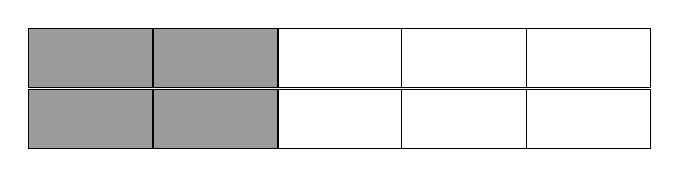
\begin{tikzpicture}[x=0.75pt,y=0.75pt,yscale=-1,xscale=1]
\draw  [fill={rgb, 255:red, 155; green, 155; blue, 155 }  ,fill opacity=1 ] (60.5,50.5) -- (120.5,50.5) -- (120.5,79) -- (60.5,79) -- cycle ;
\draw  [fill={rgb, 255:red, 155; green, 155; blue, 155 }  ,fill opacity=1 ] (121,50.5) -- (181,50.5) -- (181,79) -- (121,79) -- cycle ;
\draw   (180.5,50.5) -- (240.5,50.5) -- (240.5,79) -- (180.5,79) -- cycle ;
\draw   (240.5,50.5) -- (300.5,50.5) -- (300.5,79) -- (240.5,79) -- cycle ;
\draw   (300.5,50.5) -- (360.5,50.5) -- (360.5,79) -- (300.5,79) -- cycle ;
\draw  [fill={rgb, 255:red, 155; green, 155; blue, 155 }  ,fill opacity=1 ] (60.5,80) -- (120.5,80) -- (120.5,108.5) -- (60.5,108.5) -- cycle ;
\draw  [fill={rgb, 255:red, 155; green, 155; blue, 155 }  ,fill opacity=1 ] (121,80) -- (181,80) -- (181,108.5) -- (121,108.5) -- cycle ;
\draw   (180.5,80) -- (240.5,80) -- (240.5,108.5) -- (180.5,108.5) -- cycle ;
\draw   (240.5,80) -- (300.5,80) -- (300.5,108.5) -- (240.5,108.5) -- cycle ;
\draw   (300.5,80) -- (360.5,80) -- (360.5,108.5) -- (300.5,108.5) -- cycle ;
\end{tikzpicture} 
},
optionA={$\frac{6}{10}$},
optionB={$\frac{2}{3}$},
optionC={$\frac{4}{6}$},
optionD={$\frac{4}{10}$},
correctoption={D},
}

\begin{minipage}{\linewidth}
\hspace{1cm}
\centering
\tiny
\renewcommand{\arraystretch}{1.25}
\begin{tabular}{|M{1.2cm}|M{0.8cm}|M{0.8cm}|M{0.8cm}|M{0.8cm}|M{0.8cm}|}
\hline
Option & A (\ding{55}) & B (\ding{55}) & C (\ding{55}) & \cellcolor{cellgreen} D (\ding{51}) & E \\ 
\hline
5 A & \highno{0\%} & \highno{0\%} & \highno{24\%} & \highno{71\%} & \highno{6\%} \\ 
 \hline 
5 B & \highno{0\%} & \highno{7\%} & \highno{29\%} & \highno{64\%} & \highno{0\%} \\ \hline
\end{tabular}
\end{minipage}

\end{frame}
% \input{4. PPT/My Answer/Math/C5/117_C5M - Q6}


\begin{frame}[shrink=0.1,label=QPC5QC5M03 - DT - Q1]{Q13 [3. Fractions*]}
\vspace{-0.2cm}
\mcqtextbottomOneFour{
questionnumber={13}, 
questionTag={C5M03 – DT – Q1},  
questiontext={Find the square that has one fourth shaded portion. },
optionA={
\tikzset{every picture/.style={line width=0.75pt,scale=\scalefactor}} 
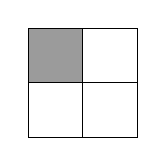
\begin{tikzpicture}[x=0.75pt,y=0.75pt,yscale=-1,xscale=1]
\draw  [fill={rgb, 255:red, 155; green, 155; blue, 155 }  ,fill opacity=1 ] (115,139.94) -- (141.28,139.94) -- (141.28,166.22) -- (115,166.22) -- cycle ;
\draw   (141.28,139.94) -- (167.57,139.94) -- (167.57,166.22) -- (141.28,166.22) -- cycle ;
\draw   (115,166.22) -- (141.28,166.22) -- (141.28,192.51) -- (115,192.51) -- cycle ;
\draw   (141.28,166.22) -- (167.57,166.22) -- (167.57,192.51) -- (141.28,192.51) -- cycle ;
\end{tikzpicture} },
optionB={
\tikzset{every picture/.style={line width=0.75pt,scale=\scalefactor}}
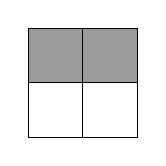
\begin{tikzpicture}[x=0.75pt,y=0.75pt,yscale=-1,xscale=1]
\draw  [fill={rgb, 255:red, 155; green, 155; blue, 155 }  ,fill opacity=1 ] (178.96,139.94) -- (205.24,139.94) -- (205.24,166.22) -- (178.96,166.22) -- cycle ;
\draw  [fill={rgb, 255:red, 155; green, 155; blue, 155 }  ,fill opacity=1 ] (205.24,139.94) -- (231.52,139.94) -- (231.52,166.22) -- (205.24,166.22) -- cycle ; 
\draw   (178.96,166.22) -- (205.24,166.22) -- (205.24,192.51) -- (178.96,192.51) -- cycle ;
\draw   (205.24,166.22) -- (231.52,166.22) -- (231.52,192.51) -- (205.24,192.51) -- cycle ;
\end{tikzpicture}},
optionC={
\tikzset{every picture/.style={line width=0.75pt,scale=\scalefactor}}
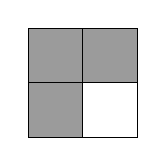
\begin{tikzpicture}[x=0.75pt,y=0.75pt,yscale=-1,xscale=1] 
\draw  [fill={rgb, 255:red, 155; green, 155; blue, 155 }  ,fill opacity=1 ] (242.91,139.94) -- (269.2,139.94) -- (269.2,166.22) -- (242.91,166.22) -- cycle ;
\draw  [fill={rgb, 255:red, 155; green, 155; blue, 155 }  ,fill opacity=1 ] (269.2,139.94) -- (295.48,139.94) -- (295.48,166.22) -- (269.2,166.22) -- cycle ;
\draw  [fill={rgb, 255:red, 155; green, 155; blue, 155 }  ,fill opacity=1 ] (242.91,166.22) -- (269.2,166.22) -- (269.2,192.51) -- (242.91,192.51) -- cycle ;
\draw   (269.2,166.22) -- (295.48,166.22) -- (295.48,192.51) -- (269.2,192.51) -- cycle ;
\end{tikzpicture}},
optionD={
\tikzset{every picture/.style={line width=0.75pt,scale=\scalefactor}} 
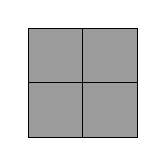
\begin{tikzpicture}[x=0.75pt,y=0.75pt,yscale=-1,xscale=1]
\draw  [fill={rgb, 255:red, 155; green, 155; blue, 155 }  ,fill opacity=1 ] (306.43,139.5) -- (332.72,139.5) -- (332.72,165.78) -- (306.43,165.78) -- cycle ;
\draw  [fill={rgb, 255:red, 155; green, 155; blue, 155 }  ,fill opacity=1 ] (332.72,139.5) -- (359,139.5) -- (359,165.78) -- (332.72,165.78) -- cycle ; 
\draw  [fill={rgb, 255:red, 155; green, 155; blue, 155 }  ,fill opacity=1 ] (306.43,165.78) -- (332.72,165.78) -- (332.72,192.07) -- (306.43,192.07) -- cycle ; 
\draw  [fill={rgb, 255:red, 155; green, 155; blue, 155 }  ,fill opacity=1 ] (332.72,165.78) -- (359,165.78) -- (359,192.07) -- (332.72,192.07) -- cycle ;
\end{tikzpicture}},
correctoption={A},
}

\begin{minipage}{\linewidth}
\hspace{1cm}
\centering
\tiny
\renewcommand{\arraystretch}{1.25}
\begin{tabular}{|M{1.2cm}|M{0.8cm}|M{0.8cm}|M{0.8cm}|M{0.8cm}|M{0.8cm}|}
\hline
Option & \cellcolor{cellgreen} A (\ding{51}) & B (\ding{55}) & C (\ding{55}) & D (\ding{55}) & E \\ 
\hline
5 A & \highno{47\%} & \highno{0\%} & \highno{6\%} & \highno{35\%} & \highno{12\%} \\ 
 \hline 
5 B & \highno{43\%} & \highno{7\%} & \highno{21\%} & \highno{29\%} & \highno{0\%} \\ \hline
\end{tabular}
\end{minipage}

\end{frame}
% \input{4. PPT/My Answer/Math/C5/117_C5M - Q13}


\begin{frame}[shrink=0.1,label=QPC5QC5M03 - DT - Q2]{Q37 [3. Fractions*]}
\vspace{-0.2cm}
\mcqtextbottomOneFour{
questionnumber={37}, 
questionTag={C5M03 – DT – Q2},  
questiontext={What is the half of 50? },
optionA={5},
optionB={50},
optionC={25},
optionD={100},
correctoption={C},
}

\begin{minipage}{\linewidth}
\hspace{1cm}
\centering
\tiny
\renewcommand{\arraystretch}{1.25}
\begin{tabular}{|M{1.2cm}|M{0.8cm}|M{0.8cm}|M{0.8cm}|M{0.8cm}|M{0.8cm}|}
\hline
Option & A (\ding{55}) & B (\ding{55}) & \cellcolor{cellgreen} C (\ding{51}) & D (\ding{55}) & E \\ 
\hline
5 A & \highno{6\%} & \highno{6\%} & \highgreen{82\%} & \highno{6\%} & \highno{0\%} \\ 
 \hline 
5 B & \highno{29\%} & \highno{0\%} & \highno{50\%} & \highno{21\%} & \highno{0\%} \\ \hline
\end{tabular}
\end{minipage}

\end{frame}
% \input{4. PPT/My Answer/Math/C5/117_C5M - Q37}


\begin{frame}[shrink=0.1,label=QPC5QC5M04 - DT - Q3]{Q9 [4. Decimals and their Conversion*]}
\vspace{-0.2cm}
\mcqtextbottomOneFour{
questionnumber={9}, 
questionTag={C5M04 – DT – Q3},  
questiontext={ Express 25 paise in rupees.},
optionA={Rs. 0.25},
optionB={Rs. 2.5},
optionC={Rs. 2500},
optionD={Rs. 25},
correctoption={A},
}

\begin{minipage}{\linewidth}
\hspace{1cm}
\centering
\tiny
\renewcommand{\arraystretch}{1.25}
\begin{tabular}{|M{1.2cm}|M{0.8cm}|M{0.8cm}|M{0.8cm}|M{0.8cm}|M{0.8cm}|}
\hline
Option & \cellcolor{cellgreen} A (\ding{51}) & B (\ding{55}) & C (\ding{55}) & D (\ding{55}) & E \\ 
\hline
5 A & \highno{41\%} & \highno{24\%} & \highno{12\%} & \highno{12\%} & \highno{12\%} \\ 
 \hline 
5 B & \highred{29\%} & \highno{36\%} & \highno{7\%} & \highno{21\%} & \highno{7\%} \\ \hline
\end{tabular}
\end{minipage}

\end{frame}
% \input{4. PPT/My Answer/Math/C5/117_C5M - Q9}


\begin{frame}[shrink=0.1,label=QPC5QC5M04 - DT - Q4]{Q14 [4. Decimals and their Conversion*]}
\vspace{-0.2cm}
\mcqtextbottomOneFour{
questionnumber={14}, 
questionTag={C5M04 – DT – Q4},  
questiontext={10 cm = \rule{80pt}{0.5pt} mm},
optionA={10 mm},
optionB={100 mm},
optionC={1 mm},
optionD={0.01 mm},
correctoption={B},
}

\begin{minipage}{\linewidth}
\hspace{1cm}
\centering
\tiny
\renewcommand{\arraystretch}{1.25}
\begin{tabular}{|M{1.2cm}|M{0.8cm}|M{0.8cm}|M{0.8cm}|M{0.8cm}|M{0.8cm}|}
\hline
Option & A (\ding{55}) & \cellcolor{cellgreen} B (\ding{51}) & C (\ding{55}) & D (\ding{55}) & E \\ 
\hline
5 A & \highno{6\%} & \highno{59\%} & \highno{29\%} & \highno{0\%} & \highno{6\%} \\ 
 \hline 
5 B & \highno{21\%} & \highno{50\%} & \highno{14\%} & \highno{7\%} & \highno{7\%} \\ \hline
\end{tabular}
\end{minipage}

\end{frame}
% \input{4. PPT/My Answer/Math/C5/117_C5M - Q14}


\begin{frame}[shrink=0.1,label=QPC5QC5M04 - DT - Q2]{Q19 [4. Decimals and their Conversion*]}
\vspace{-0.2cm}
\mcqtextbottomOneFour{
questionnumber={19}, 
questionTag={C5M04 – DT – Q2},  
questiontext={Ram bought 23.5 kg of tomatoes. Help him to represent 23.5 kg in grams. },
optionA={23500 g},
optionB={2350 g},
optionC={23.5000 g},
optionD={235 g},
correctoption={A},
}

\begin{minipage}{\linewidth}
\hspace{1cm}
\centering
\tiny
\renewcommand{\arraystretch}{1.25}
\begin{tabular}{|M{1.2cm}|M{0.8cm}|M{0.8cm}|M{0.8cm}|M{0.8cm}|M{0.8cm}|}
\hline
Option & \cellcolor{cellgreen} A (\ding{51}) & B (\ding{55}) & C (\ding{55}) & D (\ding{55}) & E \\ 
\hline
5 A & \highred{12\%} & \highno{24\%} & \highno{35\%} & \highno{24\%} & \highno{6\%} \\ 
 \hline 
5 B & \highno{50\%} & \highno{21\%} & \highno{7\%} & \highno{7\%} & \highno{14\%} \\ \hline
\end{tabular}
\end{minipage}

\end{frame}
% \input{4. PPT/My Answer/Math/C5/117_C5M - Q19}


\begin{frame}[shrink=0.1,label=QPC5QC5M04 - DT - Q7]{Q23 [4. Decimals and their Conversion*]}
\vspace{-0.2cm}
\mcqtextbottomOneFour{
questionnumber={23}, 
questionTag={C5M04 – DT – Q7},  
questiontext={Ramu has 5000 ml of water. How many 1-liter bottles will he need to hold it?},
optionA={5},
optionB={6},
optionC={55},
optionD={100},
correctoption={A},
}

\begin{minipage}{\linewidth}
\hspace{1cm}
\centering
\tiny
\renewcommand{\arraystretch}{1.25}
\begin{tabular}{|M{1.2cm}|M{0.8cm}|M{0.8cm}|M{0.8cm}|M{0.8cm}|M{0.8cm}|}
\hline
Option & \cellcolor{cellgreen} A (\ding{51}) & B (\ding{55}) & C (\ding{55}) & D (\ding{55}) & E \\ 
\hline
5 A & \highno{41\%} & \highno{12\%} & \highno{24\%} & \highno{18\%} & \highno{6\%} \\ 
 \hline 
5 B & \highno{71\%} & \highno{0\%} & \highno{14\%} & \highno{14\%} & \highno{0\%} \\ \hline
\end{tabular}
\end{minipage}

\end{frame}
% \input{4. PPT/My Answer/Math/C5/117_C5M - Q23}


\begin{frame}[shrink=0.1,label=QPC5QC5M04 - DT - Q1]{Q33 [4. Decimals and their Conversion*]}
\vspace{-0.2cm}
\mcqtextbottomOneFour{
questionnumber={33}, 
questionTag={C5M04 – DT – Q1},  
questiontext={The representation of the fraction {{$\dfrac{1}{100}$}} in decimal form is \rule{80pt}{0.5pt}},
optionA={0.1},
optionB={0.01},
optionC={0.001},
optionD={1},
correctoption={B},
}

\begin{minipage}{\linewidth}
\hspace{1cm}
\centering
\tiny
\renewcommand{\arraystretch}{1.25}
\begin{tabular}{|M{1.2cm}|M{0.8cm}|M{0.8cm}|M{0.8cm}|M{0.8cm}|M{0.8cm}|}
\hline
Option & A (\ding{55}) & \cellcolor{cellgreen} B (\ding{51}) & C (\ding{55}) & D (\ding{55}) & E \\ 
\hline
5 A & \highno{0\%} & \highgreen{88\%} & \highno{6\%} & \highno{6\%} & \highno{0\%} \\ 
 \hline 
5 B & \highno{0\%} & \highno{71\%} & \highno{29\%} & \highno{0\%} & \highno{0\%} \\ \hline
\end{tabular}
\end{minipage}

\end{frame}
% \input{4. PPT/My Answer/Math/C5/117_C5M - Q33}


\begin{frame}[shrink=0.1,label=QPC5QC5M04 - DT - Q5]{Q38 [4. Decimals and their Conversion*]}
\vspace{-0.2cm}
\mcqtextbottomOneFour{
questionnumber={38}, 
questionTag={C5M04 – DT – Q5},  
questiontext={Which unit is used to measure the quantity of water in a bucket?},
optionA={Kilometer},
optionB={Liter},
optionC={Meter},
optionD={Decigram},
correctoption={B},
}

\begin{minipage}{\linewidth}
\hspace{1cm}
\centering
\tiny
\renewcommand{\arraystretch}{1.25}
\begin{tabular}{|M{1.2cm}|M{0.8cm}|M{0.8cm}|M{0.8cm}|M{0.8cm}|M{0.8cm}|}
\hline
Option & A (\ding{55}) & \cellcolor{cellgreen} B (\ding{51}) & C (\ding{55}) & D (\ding{55}) & E \\ 
\hline
5 A & \highno{0\%} & \highgreen{88\%} & \highno{6\%} & \highno{0\%} & \highno{6\%} \\ 
 \hline 
5 B & \highno{14\%} & \highgreen{86\%} & \highno{0\%} & \highno{0\%} & \highno{0\%} \\ \hline
\end{tabular}
\end{minipage}

\end{frame}
% \input{4. PPT/My Answer/Math/C5/117_C5M - Q38}


\begin{frame}[shrink=0.1,label=QPC5QC5M04 - DT - Q6]{Q39 [4. Decimals and their Conversion*]}
\vspace{-0.2cm}
\mcqtextbottomOneFour{
questionnumber={39}, 
questionTag={C5M04 – DT – Q6},  
questiontext={Find the time duration between 9:15 AM and 11:45 AM.},
optionA={2 hours},
optionB={1.5 hours},
optionC={2.25 hours},
optionD={2.5 hours},
correctoption={D},
}

\begin{minipage}{\linewidth}
\hspace{1cm}
\centering
\tiny
\renewcommand{\arraystretch}{1.25}
\begin{tabular}{|M{1.2cm}|M{0.8cm}|M{0.8cm}|M{0.8cm}|M{0.8cm}|M{0.8cm}|}
\hline
Option & A (\ding{55}) & B (\ding{55}) & C (\ding{55}) & \cellcolor{cellgreen} D (\ding{51}) & E \\ 
\hline
5 A & \highno{29\%} & \highno{12\%} & \highno{29\%} & \highred{12\%} & \highno{18\%} \\ 
 \hline 
5 B & \highno{14\%} & \highno{21\%} & \highno{50\%} & \highred{14\%} & \highno{0\%} \\ \hline
\end{tabular}
\end{minipage}

\end{frame}
% \input{4. PPT/My Answer/Math/C5/117_C5M - Q39}


\begin{frame}[shrink=0.1,label=QPC5QC5M05 - DT - Q1]{Q21 [5. Shapes and Angles*]}
\vspace{-0.2cm}
\mcqimgleftFourOne{
questionnumber={21}, 
questionTag={C5M05 – DT – Q1}, 
questiontext={Identify the number of sides in the given figure.},
imgtabletikz = { \adjustbox{scale=\scalefactor}{\includegraphics[height= 2.5cm, width= 3.5 cm]{C5M05 – DT – Q1.png}}},
optionA={No sides},
optionB={Six sides},
optionC={Four sides},
optionD={Three sides},
correctoption={C},
leftmini={0.5},
rightmini={0.4},
}

\begin{minipage}{\linewidth}
\hspace{1cm}
\centering
\tiny
\renewcommand{\arraystretch}{1.25}
\begin{tabular}{|M{1.2cm}|M{0.8cm}|M{0.8cm}|M{0.8cm}|M{0.8cm}|M{0.8cm}|}
\hline
Option & A (\ding{55}) & B (\ding{55}) & \cellcolor{cellgreen} C (\ding{51}) & D (\ding{55}) & E \\ 
\hline
5 A & \highno{0\%} & \highno{0\%} & \highgreen{100\%} & \highno{0\%} & \highno{0\%} \\ 
 \hline 
5 B & \highno{7\%} & \highno{0\%} & \highgreen{79\%} & \highno{0\%} & \highno{14\%} \\ \hline
\end{tabular}
\end{minipage}

\end{frame}
% \input{4. PPT/My Answer/Math/C5/117_C5M - Q21}


\begin{frame}[shrink=0.1,label=QPC5QC5M05 - DT - Q3]{Q22 [5. Shapes and Angles*]}
\vspace{-0.2cm}
\mcqimgleftFourOne{
questionnumber={22}, 
questionTag={C5M05 – DT – Q3},  
questiontext={In the given figure, the angle formed is \rule{80pt}{0.5pt} the right angle. },
imgtabletikz = { \adjustbox{scale=\scalefactor}{\includegraphics[height= 3cm, width= 3 cm]{C5M05 – DT – Q3.png}}},
optionA={Equal to},
optionB={Greater than},
optionC={Lesser than},
optionD={Not equal to},
correctoption={B},
leftmini={0.6},
rightmini={0.3},
}

\begin{minipage}{\linewidth}
\hspace{1cm}
\centering
\tiny
\renewcommand{\arraystretch}{1.25}
\begin{tabular}{|M{1.2cm}|M{0.8cm}|M{0.8cm}|M{0.8cm}|M{0.8cm}|M{0.8cm}|}
\hline
Option & A (\ding{55}) & \cellcolor{cellgreen} B (\ding{51}) & C (\ding{55}) & D (\ding{55}) & E \\ 
\hline
5 A & \highno{12\%} & \highred{35\%} & \highno{29\%} & \highno{18\%} & \highno{6\%} \\ 
 \hline 
5 B & \highno{7\%} & \highred{29\%} & \highno{7\%} & \highno{43\%} & \highno{14\%} \\ \hline
\end{tabular}
\end{minipage}

\end{frame}
% \input{4. PPT/My Answer/Math/C5/117_C5M - Q22}


\begin{frame}[shrink=0.1,label=QPC5QC5M05 - DT - Q2]{Q29 [5. Shapes and Angles*]}
\vspace{-0.2cm}
\mcqimgleftFourOne{
questionnumber={29}, 
questionTag={C5M05 – DT – Q2},  
questiontext={Find the length of pencil. },
imgtabletikz = { \adjustbox{scale=\scalefactor}{\includegraphics[height= 3cm, width= 10 cm]{C5M05 – DT – Q2.png}}},
optionA={6.5 cm},
optionB={5.5 cm},
optionC={5 cm},
optionD={6 cm},
correctoption={B},
leftmini={0.6},
rightmini={0.3},
}

\begin{minipage}{\linewidth}
\hspace{1cm}
\centering
\tiny
\renewcommand{\arraystretch}{1.25}
\begin{tabular}{|M{1.2cm}|M{0.8cm}|M{0.8cm}|M{0.8cm}|M{0.8cm}|M{0.8cm}|}
\hline
Option & A (\ding{55}) & \cellcolor{cellgreen} B (\ding{51}) & C (\ding{55}) & D (\ding{55}) & E \\ 
\hline
5 A & \highno{6\%} & \highgreen{94\%} & \highno{0\%} & \highno{0\%} & \highno{0\%} \\ 
 \hline 
5 B & \highno{0\%} & \highgreen{79\%} & \highno{21\%} & \highno{0\%} & \highno{0\%} \\ \hline
\end{tabular}
\end{minipage}

\end{frame}
% \input{4. PPT/My Answer/Math/C5/117_C5M - Q29}


\begin{frame}[shrink=0.1,label=QPC5QC5M06 - DT - Q2]{Q25 [6. Visualization*]}
\vspace{-0.2cm}
\mcqimgleftFourOne{
questionnumber={25}, 
questionTag={C5M06 – DT – Q2},  
questiontext={ Identify the shape of the following image.},
imgtabletikz = { \adjustbox{scale=\scalefactor}{\includegraphics[height= 2.5 cm, width= 5 cm]{C5M06 – DT – Q2.png}}},
optionA={Cube},
optionB={Cuboid},
optionC={Cone},
optionD={Cylinder},
correctoption={C},
leftmini={0.6},
rightmini={0.3},
}

\begin{minipage}{\linewidth}
\hspace{1cm}
\centering
\tiny
\renewcommand{\arraystretch}{1.25}
\begin{tabular}{|M{1.2cm}|M{0.8cm}|M{0.8cm}|M{0.8cm}|M{0.8cm}|M{0.8cm}|}
\hline
Option & A (\ding{55}) & B (\ding{55}) & \cellcolor{cellgreen} C (\ding{51}) & D (\ding{55}) & E \\ 
\hline
5 A & \highno{0\%} & \highno{12\%} & \highgreen{88\%} & \highno{0\%} & \highno{0\%} \\ 
 \hline 
5 B & \highno{0\%} & \highno{7\%} & \highgreen{86\%} & \highno{7\%} & \highno{0\%} \\ \hline
\end{tabular}
\end{minipage}

\end{frame}
% \input{4. PPT/My Answer/Math/C5/117_C5M - Q25}


\begin{frame}[shrink=0.1,label=QPC5QC5M06 - DT - Q1]{Q28 [6. Visualization*]}
\vspace{-0.2cm}
\mcqtextbottomOneFour{
questionnumber={28}, 
questionTag={C5M06 – DT – Q1},  
questiontext={Ajaykanth got a salary of Rs.10,000 in January month, Rs.12,000 in February month, Rs. 14,000 in March month and the pattern continued. How much he had earned in the month of June? },
optionA={Rs. 18,000},
optionB={Rs. 16,000},
optionC={Rs. 15,000},
optionD={Rs. 20,000},
correctoption={D},
}

\begin{minipage}{\linewidth}
\hspace{1cm}
\centering
\tiny
\renewcommand{\arraystretch}{1.25}
\begin{tabular}{|M{1.2cm}|M{0.8cm}|M{0.8cm}|M{0.8cm}|M{0.8cm}|M{0.8cm}|}
\hline
Option & A (\ding{55}) & B (\ding{55}) & C (\ding{55}) & \cellcolor{cellgreen} D (\ding{51}) & E \\ 
\hline
5 A & \highno{12\%} & \highno{53\%} & \highno{6\%} & \highred{24\%} & \highno{6\%} \\ 
 \hline 
5 B & \highno{21\%} & \highno{36\%} & \highno{14\%} & \highred{14\%} & \highno{14\%} \\ \hline
\end{tabular}
\end{minipage}

\end{frame}
% \input{4. PPT/My Answer/Math/C5/117_C5M - Q28}


\begin{frame}[shrink=0.1,label=QPC5QC5M07 - DT - Q2]{Q3 [7. Symmetry*]}
\vspace{-0.2cm}
\mcqtextbottomOneFour{
questionnumber={3}, 
questionTag={C5M07 – DT – Q2},  
questiontext={Pick the shape which is not divided into two mirror halves by the dotted line.\\
\adjustbox{scale=\scalefactor}{\includegraphics[height= 3.5cm, width= 16 cm]{C5M07 – DT – Q2.png}}
},
optionA={i},
optionB={ii},
optionC={iii},
optionD={iv},
correctoption={B},
}

\begin{minipage}{\linewidth}
\hspace{1cm}
\centering
\tiny
\renewcommand{\arraystretch}{1.25}
\begin{tabular}{|M{1.2cm}|M{0.8cm}|M{0.8cm}|M{0.8cm}|M{0.8cm}|M{0.8cm}|}
\hline
Option & A (\ding{55}) & \cellcolor{cellgreen} B (\ding{51}) & C (\ding{55}) & D (\ding{55}) & E \\ 
\hline
5 A & \highno{6\%} & \highgreen{76\%} & \highno{12\%} & \highno{6\%} & \highno{0\%} \\ 
 \hline 
5 B & \highno{7\%} & \highgreen{79\%} & \highno{7\%} & \highno{7\%} & \highno{0\%} \\ \hline
\end{tabular}
\end{minipage}

\end{frame}
% \input{4. PPT/My Answer/Math/C5/117_C5M - Q3}


\begin{frame}[shrink=0.1,label=QPC5QC5M08 - DT - Q2]{Q11 [8. Mensuration*]}
\vspace{-0.2cm}
\mcqtextbottomOneFour{
questionnumber={11}, 
questionTag={C5M08 – DT – Q2},  
questiontext={Find the perimeter of the rectangle if its length and breadth is 10 cm and 4 cm respectively. },
optionA={14 cm},
optionB={28 cm},
optionC={40 cm},
optionD={104 cm},
correctoption={B},
}

\begin{minipage}{\linewidth}
\hspace{1cm}
\centering
\tiny
\renewcommand{\arraystretch}{1.25}
\begin{tabular}{|M{1.2cm}|M{0.8cm}|M{0.8cm}|M{0.8cm}|M{0.8cm}|M{0.8cm}|}
\hline
Option & A (\ding{55}) & \cellcolor{cellgreen} B (\ding{51}) & C (\ding{55}) & D (\ding{55}) & E \\ 
\hline
5 A & \highno{18\%} & \highno{47\%} & \highno{29\%} & \highno{6\%} & \highno{0\%} \\ 
 \hline 
5 B & \highno{21\%} & \highno{50\%} & \highno{21\%} & \highno{0\%} & \highno{7\%} \\ \hline
\end{tabular}
\end{minipage}

\end{frame}
% \input{4. PPT/My Answer/Math/C5/117_C5M - Q11}


\begin{frame}[shrink=0.1,label=QPC5QC5M08 - DT - Q3]{Q24 [8. Mensuration*]}
\vspace{-0.2cm}
\mcqimgleftFourOne{
questionnumber={24}, 
questionTag={C5M08 – DT – Q3},  
questiontext={Find the area of the rectangle. },
imgtabletikz = { 
\tikzset{every picture/.style={line width=0.75pt,scale=\scalefactor}} 
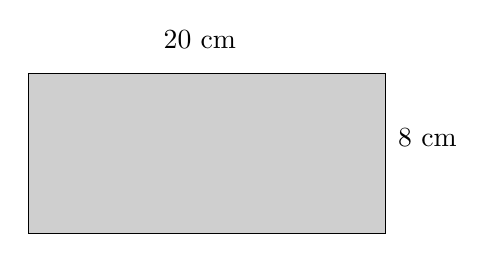
\begin{tikzpicture}[x=0.75pt,y=0.75pt,yscale=-1,xscale=1]
\draw  [fill={rgb, 255:red, 155; green, 155; blue, 155 }  ,fill opacity=0.48 ] (122,102) -- (294,102) -- (294,179) -- (122,179) -- cycle ;
\draw (186,80) node [anchor=north west][inner sep=0.75pt]   [align=left] {20 cm};
\draw (299,127) node [anchor=north west][inner sep=0.75pt]   [align=left] {8 cm};
\end{tikzpicture} },
optionA={12 sq. cm},
optionB={28 sq. cm},
optionC={56 sq. cm},
optionD={160 sq.cm},
correctoption={D},
leftmini={0.6},
rightmini={0.3},
}

\begin{minipage}{\linewidth}
\hspace{1cm}
\centering
\tiny
\renewcommand{\arraystretch}{1.25}
\begin{tabular}{|M{1.2cm}|M{0.8cm}|M{0.8cm}|M{0.8cm}|M{0.8cm}|M{0.8cm}|}
\hline
Option & A (\ding{55}) & B (\ding{55}) & C (\ding{55}) & \cellcolor{cellgreen} D (\ding{51}) & E \\ 
\hline
5 A & \highno{0\%} & \highno{24\%} & \highno{24\%} & \highno{53\%} & \highno{0\%} \\ 
 \hline 
5 B & \highno{14\%} & \highno{14\%} & \highno{0\%} & \highno{64\%} & \highno{7\%} \\ \hline
\end{tabular}
\end{minipage}

\end{frame}
% \input{4. PPT/My Answer/Math/C5/117_C5M - Q24}


\begin{frame}[shrink=0.1,label=QPC5QC5M08 - DT - Q1]{Q36 [8. Mensuration*]}
\vspace{-0.2cm}
\mcqimgleftFourOne{
questionnumber={36}, 
questionTag={C5M08 – DT – Q1},  
questiontext={Find the area of the following shaded squares, if the side of one square is 1 cm. },
imgtabletikz = { \adjustbox{scale=\scalefactor}{\includegraphics[height= 2.5cm, width= 6 cm]{C5M08 – DT – Q1.png}}},
optionA={28 sq. cm},
optionB={56 sq. cm},
optionC={14 sq. cm},
optionD={7 sq. cm},
correctoption={C},
leftmini={0.6},
rightmini={0.3},
}

\begin{minipage}{\linewidth}
\hspace{1cm}
\centering
\tiny
\renewcommand{\arraystretch}{1.25}
\begin{tabular}{|M{1.2cm}|M{0.8cm}|M{0.8cm}|M{0.8cm}|M{0.8cm}|M{0.8cm}|}
\hline
Option & A (\ding{55}) & B (\ding{55}) & \cellcolor{cellgreen} C (\ding{51}) & D (\ding{55}) & E \\ 
\hline
5 A & \highno{0\%} & \highno{0\%} & \highgreen{94\%} & \highno{0\%} & \highno{6\%} \\ 
 \hline 
5 B & \highno{7\%} & \highno{0\%} & \highgreen{86\%} & \highno{7\%} & \highno{0\%} \\ \hline
\end{tabular}
\end{minipage}

\end{frame}
% \input{4. PPT/My Answer/Math/C5/117_C5M - Q36}


\begin{frame}[shrink=0.1,label=QPC5QC5M09 - DT - Q2]{Q16 [9. Charts*]}
\vspace{-0.2cm}
\mcqimgleftFourOne{
questionnumber={16}, 
questionTag={C5M09 – DT – Q2},  
questiontext={Which genre is liked more? },
imgtabletikz = { \adjustbox{scale=\scalefactor}{\includegraphics[height= 4cm, width= 10 cm]{C5M09 – DT – Q2.png}}},
optionA={Comedy},
optionB={Horror},
optionC={Thriller},
optionD={Romance},
correctoption={A},
leftmini={0.6},
rightmini={0.3},
}

\begin{minipage}{\linewidth}
\hspace{1cm}
\centering
\tiny
\renewcommand{\arraystretch}{1.25}
\begin{tabular}{|M{1.2cm}|M{0.8cm}|M{0.8cm}|M{0.8cm}|M{0.8cm}|M{0.8cm}|}
\hline
Option & \cellcolor{cellgreen} A (\ding{51}) & B (\ding{55}) & C (\ding{55}) & D (\ding{55}) & E \\ 
\hline
5 A & \highgreen{100\%} & \highno{0\%} & \highno{0\%} & \highno{0\%} & \highno{0\%} \\ 
 \hline 
5 B & \highgreen{100\%} & \highno{0\%} & \highno{0\%} & \highno{0\%} & \highno{0\%} \\ \hline
\end{tabular}
\end{minipage}

\end{frame}
% \input{4. PPT/My Answer/Math/C5/117_C5M - Q16}


\begin{frame}[shrink=0.1,label=QPC5QC5M09 - DT - Q1]{Q40 [9. Charts*]}
\vspace{-0.2cm}
\mcqtextbottomOneFour{
questionnumber={40}, 
questionTag={C5M09 – DT – Q1},  
questiontext={Find the number for the tally mark representation of \tikzset{every picture/.style={line width=0.75pt,scale=\scalefactor}} 
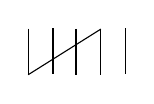
\begin{tikzpicture}[x=0.75pt,y=0.75pt,yscale=-1,xscale=1] 
\draw    (98.33,161.14) -- (98.33,183.39) ;
\draw    (110.28,161) -- (110.28,183.25) ;
\draw    (121.36,161.28) -- (121.36,183.53) ;
\draw    (133.31,161.42) -- (133.31,183.67) ;
\draw    (133.31,161.42) -- (98.33,183.39) ;
\draw    (145.26,161) -- (145.26,183.25) ;
\end{tikzpicture} },
optionA={8},
optionB={6},
optionC={7},
optionD={5},
correctoption={B},
}

\begin{minipage}{\linewidth}
\hspace{1cm}
\centering
\tiny
\renewcommand{\arraystretch}{1.25}
\begin{tabular}{|M{1.2cm}|M{0.8cm}|M{0.8cm}|M{0.8cm}|M{0.8cm}|M{0.8cm}|}
\hline
Option & A (\ding{55}) & \cellcolor{cellgreen} B (\ding{51}) & C (\ding{55}) & D (\ding{55}) & E \\ 
\hline
5 A & \highno{6\%} & \highno{71\%} & \highno{0\%} & \highno{24\%} & \highno{0\%} \\ 
 \hline 
5 B & \highno{14\%} & \highno{64\%} & \highno{0\%} & \highno{7\%} & \highno{14\%} \\ \hline
\end{tabular}
\end{minipage}

\end{frame}
% \input{4. PPT/My Answer/Math/C5/117_C5M - Q40}


\begin{frame}[shrink=0.1,label=QPC5QC6M17 - DT - Q8]{Q8 [17. Data Handling *]}
\vspace{-0.2cm}
\mcqimgleftFourOne{
questionnumber={8}, 
questionTag={C6M17 – DT – Q8}, 
questiontext={Find the day in which the least number of fruits are sold.},
imgtabletikz = { 
\adjustbox{scale=\scalefactor}{\includegraphics[width=13cm, height=6.5cm]{C6M17 - DT - Q3.png}}},
optionA={Monday},
optionB={Wednesday},
optionC={Friday},
optionD={Saturday},
leftmini={0.65},
rightmini={0.25},
correctoption={A},
}

\begin{minipage}{\linewidth}
\hspace{1cm}
\centering
\tiny
\renewcommand{\arraystretch}{1.25}
\begin{tabular}{|M{1.2cm}|M{0.8cm}|M{0.8cm}|M{0.8cm}|M{0.8cm}|M{0.8cm}|}
\hline
Option & \cellcolor{cellgreen} A (\ding{51}) & B (\ding{55}) & C (\ding{55}) & D (\ding{55}) & E \\ 
\hline
5 A & \highgreen{82\%} & \highno{0\%} & \highno{0\%} & \highno{18\%} & \highno{0\%} \\ 
 \hline 
5 B & \highgreen{79\%} & \highno{7\%} & \highno{0\%} & \highno{14\%} & \highno{0\%} \\ \hline
\end{tabular}
\end{minipage}

\end{frame}
% \input{4. PPT/My Answer/Math/C5/117_C5M - Q8}


\begin{frame}[shrink=0.1,label=QPC5QC6M17 - DT - Q2]{Q34 [17. Data Handling *]}
\vspace{-0.2cm}
\mcqimgleftFourOne{
questionnumber={34}, 
questiontext={Observe the given pictograph and find the number of roses sold on Thursday.},
imgtabletikz  = {
\renewcommand{\arraystretch}{1.25}
\begin{tabular}{|c|c|}
\hline
  Days & Number of roses sold (1 \smiley = 1 rose)  \\
  \hline
  Monday& \smiley \smiley \smiley  \\
  \hline
  Tuesday  & \smiley \smiley \smiley \smiley \smiley \smiley \smiley  \\
  \hline
  Wednesday & \smiley \smiley \smiley \smiley \smiley \smiley \smiley \smiley \\
  \hline
  Thursday & \smiley \smiley \smiley \smiley \smiley \smiley \\
  \hline
\end{tabular}  },
optionA={0},
optionB={8},
optionC={6},
optionD={7},
questionTag={C6M17 - DT - Q2}, 
leftmini={0.5},
rightmini={0.3},
correctoption={C},
}

\begin{minipage}{\linewidth}
\hspace{1cm}
\centering
\tiny
\renewcommand{\arraystretch}{1.25}
\begin{tabular}{|M{1.2cm}|M{0.8cm}|M{0.8cm}|M{0.8cm}|M{0.8cm}|M{0.8cm}|}
\hline
Option & A (\ding{55}) & B (\ding{55}) & \cellcolor{cellgreen} C (\ding{51}) & D (\ding{55}) & E \\ 
\hline
5 A & \highno{0\%} & \highno{0\%} & \highgreen{94\%} & \highno{6\%} & \highno{0\%} \\ 
 \hline 
5 B & \highno{7\%} & \highno{7\%} & \highno{57\%} & \highno{29\%} & \highno{0\%} \\ \hline
\end{tabular}
\end{minipage}

\end{frame}
% \input{4. PPT/My Answer/Math/C5/117_C5M - Q34}

%

    